% Template for ICASSP-2018 paper; to be used with:
%          spconf.sty  - ICASSP/ICIP LaTeX style file, and
%          IEEEbib.bst - IEEE bibliography style file.
% --------------------------------------------------------------------------
\documentclass{article}
\usepackage{spconf,amsmath,graphicx}
\usepackage{array,tabu}

% Example definitions.
% --------------------
\def\x{{\mathbf x}}
\def\L{{\cal L}}

\DeclareMathOperator{\sinc2}{sinc^2}
\DeclareMathOperator*{\argmin}{arg\,min}

% Title.
% ------
\title{
OPTIMAL SPECTRAL ESTIMATION AND SYSTEM TRADE-OFF IN LONG-DISTANCE FREQUENCY-MODULATED CONTINUOUS-WAVE LIDAR
}
%
% Single address.
% ---------------
\name{Taehwan Kim, Pavan Bhargava and Vladimir Stojanovi\'{c}
% \thanks{Thanks to XYZ agency for funding.}
}
\address{Department of Electrical Engineering and Computer Sciences, University of California, Berkeley, USA}

% For example:
% ------------
%\address{School\\
%	Department\\
%	Address}
%
% Two addresses (uncomment and modify for two-address case).
% ----------------------------------------------------------
%\twoauthors
%  {A. Author-one, B. Author-two\sthanks{Thanks to XYZ agency for funding.}}
%	{School A-B\\
%	Department A-B\\
%	Address A-B}
%  {C. Author-three, D. Author-four\sthanks{The fourth author performed the work
%	while at ...}}
%	{School C-D\\
%	Department C-D\\
%	Address C-D}
%
\graphicspath {{figures/}}

\begin{document}
\ninept

\maketitle

\begin{abstract}
Frequency-modulated continuous-wave (FMCW) LIDAR is a promising technology for next-generation integrated 3D imaging system. However, it has been considered to be difficult to apply for long-distance (\textgreater 100m) targets since maintaining coherence between reflected beam from the target and locally forwarded beam becomes a significant challenge for tunable laser design. This paper demonstrates the possibility of extending the detection range of FMCW LIDAR beyond the coherence range of its laser by improving the spectral estimation algorithm. By exploiting the Lorentzian prior of the receiver signal in the spectral domain, \textgreater 10x improvement in ranging accuracy was possible compared to traditional algorithms that does not consider phase noise in the signal model. In light of this finding, the end-to-end modeling framework is presented to reveal true system-level trade-off of FMCW LIDAR and the feasibility of long-distance measurement.

% evaluates the impact of spectral estimation scheme in the frequency-modulated continuous-wave (FMCW) LIDAR systems, particularly focusing on the long-distance targets where the coherence between reflected beam from the target and locally forwarded beam is no longer guaranteed. It is commonly believed that in FMCW LIDAR the target must be within the coherence range, imposing a constraint which significantly limits the tolerable linewidth of the the tunable laser. By 
% exploiting Lorentzian shape of the LIDAR signal in incoherent regime, it is possible to achieve \textgreater 10x improvement in ranging accuracy compared to simple peak-finding. Based on this finding and using end-to-end system model with realistic numbers, we 

% The abstract should appear at the top of the left-hand column of text, about
% 0.5 inch (12 mm) below the title area and no more than 3.125 inches (80 mm) in
% length.  Leave a 0.5 inch (12 mm) space between the end of the abstract and the
% beginning of the main text.  The abstract should contain about 100 to 150
% words, and should be identical to the abstract text submitted electronically
% along with the paper cover sheet.  All manuscripts must be in English, printed
% in black ink.

\end{abstract}

\begin{keywords}Frequency-modulated continuous-wave (FMCW) LIDAR, remote sensing, 3D imaging, spectral estimation
\end{keywords}

\section{Introduction}
\label{sec:intro}

Using light as the sensing medium, LIDAR (light detection and ranging) can achieve orders-of-magnitude superior lateral resolution compared to ultrasound or RF wave-based 3D imaging systems of similar form-factor and thus considered as a crucial building block for autonomous vehicles or smart robots \cite{autonomouscar}\cite{smartrobot}. Especially, frequency-modulated continuous-wave (FMCW) LIDAR has strong advantage for such applications over time-of-flight (TOF) LIDAR, largely due to its compatibility with existing integrated electro-optics platform.

% and immunity to ambient light or interferences \cite{Lamp86}.

In FMCW LIDAR, the depth information is captured by the spectral content of the photocurrent signal at the coherent receiver. This implies that the quality of the receiver signal is a function of the spectral purity of the laser source. Beyond the coherence range of the laser, which is inversely proportional to the laser linewidth, the receiver signal exhibits Lorentzian power spectral density (PSD) instead of the clean beating tone. As a result, it is commonly assumed that FMCW measurement is not possible for the range beyond the coherence range of the laser. With that constraint, producing frequency-modulated laser signal with high spectral purity for long-distance (\textgreater 100m) FMCW LIDAR relevant to automotive or airborne applications becomes highly challenging.

% the phase noise of the reflected beam from the target and that of locally forwarded beam are no longer correlated and 
% Some practical numbers for commercial laser linewidth

Even beyond the coherence range, it is still possible to carry out the distance measurement, just with degraded accuracy. Many works on FMCW RADAR, the same ranging method implemented using RF wave instead of laser, analyzed the general impact of the phase noise on the ranging performance. \cite{C2} measured the sensitivity of frequency estimation accuracy with respect to the sinusoidal phase noise so that the relationship between given phase noise profile and the ranging performance can be quantified. \cite{C2} studied the impact of phase noise in more general system context and verified their analysis with measurement results. However, it all used simple periodogram-based method as their frequency estimation algorithm. Even though there are a few frequency estimation algorithms proposed for improving ranging accuracy of FMCW measurements\cite{C2}\cite{C2}, none of them attempted to modify the algorithm to address the phase noise. Moreover, system-level study including the impact of algorithm choice is lacking.

% Also, from extensive studies on the general characteristics of the signal at the receiver in presence of laser phase noise, \cite{Lamp86} the expression for the PSD of the receiver signal is well known. However, such knowledge has not been fully exploited for the detection algorithm. 

% mention some FMCW radar papers

% Indeed, one of the biggest challenges for extending the FMCW LIDAR range to long-distance (\textgreater 100m) is the difficulty of building the laser whose wavelength can be continuously tuned over wide range while having linewidth narrow enough to maintain coherence for such distant targets. 

% for the design of spectral estimation algorithm is extremely critical. /
% making it possible to achieve reasonable performance for targets well beyond the coherence range. 
 
In this work, we first propose a spectral estimation algorithm optimized for incoherent FMCW LIDAR measurement. By leveraging known Lorentzian prior of the receiver signal in the spectral domain, the accuracy was improved by \textgreater 10x, making it possible to achieve reasonable performance for targets well beyond the coherence range. Based on this concept, we also present our end-to-end model for FMCW LIDAR including the spectral estimation method to map the system specifications to the ranging accuracy. Using this model, we provide a guideline for FMCW LIDAR link budget analysis so that one can estimate required laser power and receiver bandwidth for given system parameters and accuracy/range target.

The remainder of the paper is organized as follows. Section 2 provides an overview of the operating principle of FMCW LIDAR. In Section 3, the impact of phase noise in the laser on FMCW measurement is studied. Section 4 introduces proposed spectral estimation scheme leveraging the PSD prior in presence of the phase noise. Section 5 finally presents the end-to-end model for FMCW LIDAR system including the spectral estimation algorithm and provides the system design guideline based on this model. Section 6 concludes the paper.
%  and shows its impact on the LIDAR performanc

\section{FMCW LIDAR CONCEPT}
\label{sec:fmcw}

Overview of the FMCW LIDAR system is shown in Fig. 1. At the core of FMCW LIDAR is continuous-wave tunable laser whose frequency is modulated using certain waveform, as its name suggests. Despite that it is possible to use various types of the modulation waveform, we only consider the case of sawtooth wave in this paper. Over the observation time $T$, frequency of the laser is linearly increased by the chirp bandwidth $f_\text{BW}$. Resulting modulated laser with chirping rate $\gamma=f_\text{BW}/T$ is split into two beams. One beam goes into the free space directed towards the target of interest, and gets reflected. The other beam stays in the sensor, going directly into the coherent receiver ($E_\text{LO}$) along with the beam collected from the reflection ($E_\text{RX}$). 

% \begin{align}
% \phi_{pc}(t) &= \phi_{RX}(t)-\phi_{LO}(t) \\
% &= (\omega_{RX}(t)-\omega_{LO}(t))t+\phi_{RX}(t)-\phi_{LO}(t)
% \end{align}
Due to the group delay mismatch between two beams, there is a instantaneous frequency difference, as shown in Fig. 1(b). The coherent receiver acts as an analog mixer and produces the photocurrent whose frequency $f_\text{beat}$ is equal to this difference. It is obvious from Fig. 1(b) that $f_\text{beat}$ is directly proportional to both $\gamma$ and the delay mismatch $\tau$. Since the delay mismatch is a linear function of the round-trip time of the reflected beam, we can measure the distance of the remote target $d$ from this beat frequency. Assuming on-chip propagation delay is negligible compared to the free-space propagation, we can simplify the relationship between $d$ and $f_\text{beat}$ with speed of light $c$ as follows.
\begin{equation}
f_\text{beat} = \gamma\tau = \frac{f_\text{BW}}{T}\frac{2d}{c}
\end{equation}

\begin{figure}[t!]
\begin{minipage}[b]{1.0\linewidth}
  \centering
  \centerline{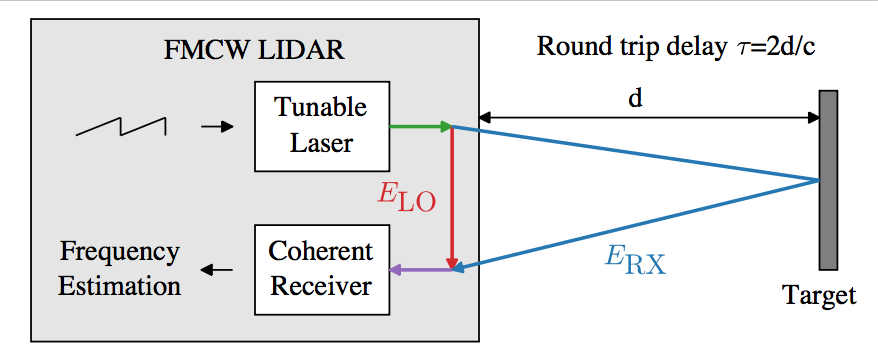
\includegraphics[width=0.9\textwidth]{fig1a}}
%   \vspace{-0.5em}
%   \centerline{(a)}\medskip
%   \vspace{-0.5em}
\end{minipage}
\begin{minipage}[b]{1.0\linewidth}
  \centering
  \centerline{\includegraphics[width=0.9\textwidth]{fig1b}}
%   \vspace{-0.5em}
%   \centerline{(b)}\medskip
  \vspace{-0.5em}
\end{minipage}
\caption{FMCW LIDAR overview}
  \vspace{-1em}
\label{fig:overview}
\end{figure}

FMCW LIDAR is particularly attractive for monolithic implementation since its building blocks are readily available in silicon photonics technology. For example, coherent detection achieves shot-noise limited performance without avalanche photodiodes unlike time-of-flight (TOF) LIDAR. In addition, it is easily extended to velocity detection through Doppler measurement, and the detection is relatively insensitive to the interference from other sensors or ambient light. Recent demonstrations of integrated FMCW LIDAR shows its potential as a baseline technology for low-cost, chip-scale 3D imaging system.

% Among many advantages of-cc-c FMCW LIDAR over more common pulse-based time-of-flight (TOF) LIDAR are 


\section{COHERENCE IN FMCW LIDAR MEASUREMENT}
\label{sec:psd}

% Assuming ideal laser, the photocurrent signal at the coherent receiver should be pure sinusoidal beating tone of frequency $f_\text{beat}$ as the receiver merely maps the phase difference between reflected beam and the local beam to the phase of the photocurrent. On top of that, receiver frontend adds noise to the measurement which is usually dominated by photodetector shot noise in coherent receivers. 

% Different from the ideal case where ideal laser 

The photocurrent signal at the coherent receiver is pure sinusoidal tone only when the phase offset of the laser is constant. In reality, the phase or frequency of any practical laser is a random process, and its randomness is quantified by full-width at half-maximum (FWHM) of the baseband spectrum of the electric field, often referred to as linewidth $\Delta\nu$. Assuming whiteness of the frequency noise, power spectral density of the laser frequency noise $\dot{\phi_n}$ is equal to its linewidth. 
\begin{equation}
S_{\dot{\phi_n}}(\omega) = \Delta\omega = 2\pi\Delta\nu
\end{equation}
Given non-zero linewidth, the phase of the photocurrent at the receiver is also a random process and its noise process is directly related to the laser phase noise by following relationship.
\begin{equation}\label{eq:pnoise}
\phi_{n, \text{photocurrent}} = \phi_{n,\text{LO}}(t)-\phi_{n,\text{RX}}(t) = \phi_n(t)-\phi_n(t-\tau)
\end{equation}
Resulting power spectral density $S_i(\omega)$ of the photocurrent signal for observation time $T$ and delay mismatch $\tau$ in shot-noise limited receiver is expressed as follows.
\begin{equation}\label{eq:psd}
S_{i}(\omega)=\frac{1}{4}\left[S_i^\circ(\omega-2\pi \gamma\tau)+S_i^\circ(\omega+2\pi \gamma\tau)\right]
\end{equation}
\begin{equation}\label{eq:psdbb}
\begin{split}
S_{i}^\circ & (\omega) = R_\text{PD}^2 P_\text{RX} P_\text{LO} \left[T \sinc2\left(\frac{T\omega}{2}\right) e^{-\frac{2\tau}{\tau_c}} + \frac{\tau_c}{1+\left(\frac{\omega\tau_c}{2}\right)^2}\right. \\ 
&\left.\cdot\left\{1-e^{-\frac{2\tau}{\tau_c}}\left[ \cos(\omega\tau) + \frac{2}{\omega\tau_c}\sin(\omega\tau) \right] \right\} + \frac{2q}{R_\text{PD}P_\text{RX}} \right]
\end{split}
\end{equation}
$R_\text{PD}$ is the responsivity of photodetector, $q$ is electron charge, and $P_{\text{RX/LO}}$ is the power of RX/LO beam. The first term in (\ref{eq:psdbb}) is the main beating tone convolved with sinc-squared function due to finite observation, and the second term forms pedestal-like distribution around the main beat tone. The last term represents shot-noise floor, which becomes more pronounced when $P_\text{RX}$ is weak. $\tau_c=2/\Delta\omega$ is coherence time of the laser, commonly used metric in the literature. This expression is assuming that the observation time $T$ is much larger than $\tau$ and $\tau_c$, which is usually the case for FMCW measurements.

When the target is close to the sensor and $\tau$ is small, the phase noise process of RX and LO beam are highly correlated. In such \textit{coherent} regime, two processes tend to cancel each other in the photocurrent phase, as shown in (\ref{eq:pnoise}). Indeed, when $\Delta\omega\tau\ll 1$, the second term in (\ref{eq:psdbb}) vanishes and the sensor gets clean, strong beating tone. On the other hand, if the target is far away ($\Delta\omega\tau\gg 1$), (\ref{eq:psdbb}) converges into following form.
\begin{equation}\label{eq:psdincoherent}
S_{i}^\circ(\omega) = R_\text{PD}^2 P_\text{RX} P_\text{LO} \left[\frac{2\Delta\omega}{\omega^2+\Delta\omega^2} + \frac{2q}{R_\text{PD}P_\text{RX}} \right]
\end{equation}
The PSD now exhibits Lorentzian shape around $f_\text{beat}$ with linewidth $2\Delta\nu$, two times the original linewidth as the phase noise power simply adds up if two beams are \textit{incoherent}.

% The target distance up to which the beams stay coherent is called coherence range and defined as following.
% \begin{equation}
% d_c = \frac{c}{\Delta\omega}
% \end{equation}

\begin{figure}[t!]
\begin{minipage}[b]{1.0\linewidth}
  \centering
  \centerline{\includegraphics[width=0.9\textwidth]{fig2}}
%   \vspace{-0.5em}
%   \centerline{(a)}\medskip
  \vspace{-1em}
\end{minipage}
\caption{Signal peak magnitude of the FMCW LIDAR signal for different target distance (left) and corresponding PSD in the frequency domain. Power density was normalized to the peak at zero distance and shot noise was ignored ($T=$10$\mu$s, $\Delta\nu=$1MHz).}
  \vspace{-1em}
\label{fig:psd}
\end{figure}

Fig. 2 shows the relationship between the distance of the target and the PSD peak power density. Shot noise floor is neglected to emphasize the impact of phase noise and the power is normalized by the beating tone at zero distance. For short distance, peak power follows the first term in (\ref{eq:psdbb}) and decays exponentially as distance goes up. This trend gradually diminishes as the second term takes over, and eventually becomes indifferent to the target distance as in (\ref{eq:psdincoherent}). This crossing point between the beating tone and the peak of the Lorentzian pedestal, or the coherence range $d_c$ relevant to FMCW measurement, is expressed as follows.
\begin{equation}\label{eq:coherentcrossing}
d_c = \frac{c\tau_c}{4}\ln{\left(\frac{T}{\tau_c}\right)}
\end{equation}
Note that it is also a function of $T$; the measurement enters incoherent regime more quickly for shorter observations.

In previous works, it has been believed that the detection range of the FMCW LIDAR is fundamentally limited by $d_c$. This is challenging for the laser design in the context of long-distance, fast-scanning LIDAR relevant to automotive applications. For the 100m range with 10$\mu$s observation time, the laser linewidth is required to be a few hundreds of kHz or less, which is difficult to guarantee especially when the laser should also be equipped with wavelength tuning. Any technique enabling fast, continuous tuning over wide wavelength range for compact lasers, such as MEMS mirror or embedded DBR, comes with significant additive phase noise. Alternatively, chirped laser can be generated using continuous-wave laser driven by an external I/Q modulator. However, it is not trivial to integrate IQ modulator, and it requires high-speed drivers and chirp generator in the electrical domain that can also add phase noise. As a result, integrated FMCW LIDAR demonstrations have been limited to short-distance measurements.

% For example, $d_c$ is only around 80m for 1MHz linewidth and 10$\mu$s observation. 

Even though the signal spectrum is in different shape and relatively weak in incoherent regime, the PSD of the photocurrent is still a function of the target distance as it is evident in (\ref{eq:psd}) and (\ref{eq:psdbb}). Moreover, we have the information from (\ref{eq:psdincoherent}) that the PSD corresponding to a target is Lorentzian in the baseband, which is still the case even without whiteness assumption for the laser frequency noise \cite{C2}. Motivated by those observations, we leverage such knowledge in the spectral estimation scheme and evaluate the FMCW LIDAR performance in incoherent regime in the next section.

% Apart from the phase noise, laser tuning nonlinearity can cause spectral leakage, degrading the SNR. However, it is possible to linearize the wavelength using feedback control. \cite{}

% In fact, the ratio of the peak power density for coherent and the incoherent case is given as $T/\tau_c$; if T becomes so short that it is comes closer to $\tau_c$, the peak power stays relatively high beyond the coherence range.

\section{SPECTRAL ESTIMATION ALGORITHM FOR LONG-DISTANCE MEASUREMENT}
\label{sec:algorithm}

All existing FMCW LIDAR works assume that the system is operating in the deep-coherent regime. Then, the phase offset of the sinusoid corresponding each target may be unknown but is constant for single observation. Since it is reasonable to assume that the number of reflective targets in one measurement is finite, the role of receiver backend is to solve classical problem of line spectra estimation. It is one of the most well-studied topics in signal processing, and there are numerous algorithms one can choose depending on the nature of additive noise or affordable complexity. In general, it is possible to achieve arbitrary accuracy as long as signal-to-noise ratio (SNR) is sufficiently high.
% $P_\text{RX}$ is high.

% In the signal model that is commonly used for line spectra estimation, the phase offset of the sinusoid may be unknown, but constant for single observation. 

On the other hand, constant phase offset assumption is invalid for FMCW measurement in incoherent regime. In \cite{C2}, it was shown that any algorithm designed assuming constant phase offset performs poorly in presence of the phase noise. Also, the lower bound of frequency estimation accuracy became a function of the phase noise, not the SNR from additive noise at the measurement. In other words, it may not be possible to achieve desired accuracy with classic frequency estimation methods even if the sensor can afford infinite power from the reflection ($P_\text{RX}$).

% common estimation method for photocurrent spectrum has been simple periodogram. From this periodogram PSD estimate, the backend simply picks the frequency bin with the highest value to determine the beat frequency and ultimately target distance. In such case, the distance measurement is mainly limited by the DFT bin-size ($\Delta f = 1/T$), and the distance error becomes a function of chirp bandwidth. 
% \begin{equation}\label{eq:fftacc}
% \epsilon_d = \frac{1}{T}\frac{cT}{2f_\text{BW}} = \frac{c}{2f_\text{BW}}
% \end{equation}
% It is also possible to even super-resolve beyond the bin size as the number of targets is finite and sparse spectrum assumption is valid.

\begin{figure}[t!]
\begin{minipage}[b]{1.0\linewidth}
  \centering
  \centerline{\includegraphics[width=0.9\textwidth]{fig3a}}
  \vspace{-0.5em}
  \centerline{(a)}\medskip
  \vspace{-0.5em}
\end{minipage}
\begin{minipage}[b]{1.0\linewidth}
  \centering
  \centerline{\includegraphics[width=0.9\textwidth]{fig3b}}
  \vspace{-0.5em}
  \centerline{(b)}\medskip
  \vspace{-0.5em}
\end{minipage}
\begin{minipage}[b]{1.0\linewidth}
  \centering
  \centerline{\includegraphics[width=0.9\textwidth]{fig3c}}
  \vspace{-0.5em}
  \centerline{(c)}\medskip
   \vspace{-1em}
\end{minipage}
\caption{Impact of frequency estimation algorithm on FMCW measurement. Distance estimation variance for different algorithms and periodogram PSD estimates are shown for (a) $(P_\text{RX},\,\Delta\nu)=(\text{1mW},\,\text{1MHz})$ (b) $(P_\text{RX},\,\Delta\nu)=(\text{1nW},\,\text{1MHz})$ (c) $(P_\text{RX},\,\Delta\nu)=(\text{1nW},\,\text{10MHz})$}
  \vspace{-1em}
\label{fig:res}
\end{figure}


In order to improve the performance of distance estimation in incoherent regime, we devised a new frequency estimation algorithm that exploits prior knowledge about the PSD shape. From (\ref{eq:psd}) and (\ref{eq:psdincoherent}), it is evident that each target shows up in the spectral domain as a Lorentzian function shifted by the beating frequency. Therefore, we can define the signal model of the single-sided power spectral density of any incoherent FMCW measurement as following.
\begin{equation}\label{eq:signalmodel}
\tilde{S}(\omega; \alpha, \omega_\text{beat}) = \sum_{i=1}^{n}{\frac{\alpha_i \Delta\omega}{(\omega-\omega_{\text{beat},i})^2+\Delta\omega^2}}+2qR_\text{PD}P_\text{LO}
\end{equation}
If the number of targets is assumed to be $n$, there are $2n$ parameters: $\omega_{\text{beat},i}$ and $\alpha_i$ are the center frequency and relative power of the $i$th Lorentzian, respectively. Given this model and periodogram estimate of the PSD from the measurement, we can simply perform nonlinear least-squares  to estimate those parameters. 
\begin{equation}\label{eq:nls}
\hat{\alpha},\hat{\omega_\text{beat}} = \argmin_{\alpha,\omega_\text{beat}}{\left|S(\omega)-\tilde{S}(\omega; \alpha, \omega_\text{beat})\right|^2}
\end{equation}
Note that the PSD itself is deterministic, but its estimate using periodogram adds uncertainty. It can also have small bias if the length of the measurement is too small, but it is generally negligible considering realistic sample rate and the observation time.

In order to test the performance of proposed Lorentzian least squares estimation (LLSE) and compare it to standard frequency estimation algorithms with constant phase offset model, we built behavioral model of FMCW LIDAR using Simulink and ran transient simulation to generate realistic data. We have assumed the $E_\text{LO}$ beam is strong enough that the receiver is shot-noise limited, and there is only one target in the measurement. Baseline laser parameters were as following: $f_\text{BW}=\text{10GHz}$, $T=\text{10}\mu\text{s}$, $\Delta\nu=\text{1MHz}$. This corresponds to $\gamma=\text{1GHz/}\mu\text{s}, d_c=\text{82.3m}, \tau_c=\text{0.318}\mu\text{s}$. Photodetector responsivity was 1A/W. With simulated time-domain measurement data for target distance up to 100m, we applied different algorithms including proposed method to estimate the distance and recorded estimation variance from 100 Monte Carlo simulations per each target distance. Among a number of constant-phase frequency estimation methods, Rife and Boorstyn's algorithm \cite{Lamp86} and MUSIC \cite{Lamp86} were used for comparison.

Fig. 3(a) shows the result when $P_\text{RX}$ is 1mW. Estimated PSD shows that the shot noise floor is almost negligible compared to the Lorentzian noise pedestal. Such high SNR is expected for short-distance targets with high reflectivity. In this case, the performance of MUSIC algorithm was the best, and proposed LLSE showed similar, but slightly worse performance. The accuracy of R\&B algorithm was roughly x worse than other algorithms except for very short distance. In contrast, $P_\text{RX}$ was set to be 1nW in Fig. 3(b). Such low SNR is more relevant assumption for long-distance LIDAR since the reflection beam undergoes significant loss during free-space propagation. Under this setting, performance of LLSE and R\&B were almost unchanged, but the MUSIC algorithm performed very poorly compared to high SNR case. This is not surprising since frequency estimation algorithms based on eigendecomposition of autocorrelation matrix, including MUSIC, relies heavily on the whiteness assumption of the additive noise model. For both high SNR and low SNR case, proposed LLSE algorithm showed consistently great performance. 

Finally, linewidth of the laser was increased to 10MHz in Fig. 3(c). Coherence range is only 10m in this case, and the measured PSD clearly shows that $E_\text{LO}$ and $E_\text{RX}$ are completely incoherent. With this noisy laser and low SNR, proposed LLSE was the only algorithm that can yield acceptable performance. For 100m target, the variance of LLSE estimator was 4.82cm in contrast to 56cm of R\&B estimation, showing \textgreater 10x improvement. From this result, we can clearly see that the impact of the frequency estimation algorithm choice for the system is critical, especially for low SNR, long-distance targets. 

% single-target comparison
% multi-target

% fmcw radar analysis papers
% zero-crossing time method
% CRLB

\section{END-TO-END FMCW LIDAR MODEL}
\label{sec:experiment}



Based on the observation so far, we used end-to-end modeling framework including the frequency estimation algorithm to reveal the system level trade-off of the FMCW LIDAR. Table 1 summarizes the list of constraints and baseline design variables for our model. Note that the maximum chirping bandwidth is limited by the receiver bandwidth here, as the fastest tone corresponding to the maximum target distance should still be within the receiver bandwidth. Even though it is also possible that the maximum chirping bandwidth is limited by the tuning range of the laser itself, for long-distance LIDAR, it is usually the receiver that limits the chirping bandwidth.

Using a behavioral model with these parameters, we evaluated the measurement accuracy at the maximum distance for different linewidth and receiver power. The result corresponding to the baseline parameters is shown on the left plot in Fig. 4. We clipped the worst-case measured accuracy to 10cm so that the region fail to meet the target accuracy is easily recognized with yellow color. It is clearly seen that larger linewidth requires higher $P_\text{RX}$ to meet the accuracy target. Also, for linewidth close to 10MHz, it can be seen that no matter how much power the sensor have from the target, it is not possible to achieve 10cm accuracy due to fundamental limit from the phase noise.

Then, we increased the receiver bandwidth to 1.5GHz. As explained, this directly relaxes maximum chirping bandwidth by the same factor, which can now be 7.5GHz, and the also the chirping rate. The simulation result is shown in the middle plot in Fig. 4, and it can be seen that the measurement is now possible for wider range of linewidth beyond 10MHz, as long as enough power is received from the target. Increasing chirping rate means the same difference in distance is mapped to bigger difference in beat frequency, and therefore we can expect better accuracy for the same noise level.

buried completely under the shot noise limit!

Finally, we reduced the target detection range to 100m, and the result is shown in the right plot in Fig. 4. By reducing the target range the worst-case SNR itself is improved as the largest $\tau$ is now three times smaller. In addition, as the fastest beating frequency is also three times smaller, we can increase the laser chirp bandwidth for the same receiver bandwidth. 

Also, we would like to emphasize again that proposed Lorentzian LSE algorithm was used for all of results shown here. The operation of the FMCW LIDAR over this linewidth and receiver power range for specified target accuracy was completely impossible with both R\&B and MUSIC algorithm.


\begin{table}[!t]
\caption{Baseline system specification and device parameters}
\vspace{1em}
\label{tbl1}
\centering
\begin{tabu} to 0.9\linewidth { X[c] X[c] }
\hline
 Ranging accuracy & \textless 10cm \\   
 \hline
 Scanning time & 10$\mu$s \\ 
 \hline
 Frequency estimation & Lorentzian LSE \\ 
 \hline
 Photodetector responsivity & 1A/W \\   
 \hline
  Receiver bandwidth & 1GHz \\ 
 \hline
  Detection range & 300m \\   
 \hline
  Max. Chirping bandwidth & 5GHz \\  
 \hline
%  \hline

%  Linewidth & 1MHz \\  
\end{tabu}
\end{table}

\begin{figure}[t!]
\begin{minipage}[b]{1.0\linewidth}
  \centering
  \centerline{\includegraphics[width=\textwidth]{fig4}}
%   \vspace{-0.5em}
%   \centerline{(a)}\medskip
%   \vspace{-0.5em}
\end{minipage}
\caption{FMCW LIDAR performance for three different system constraint (target range and the receiver bandwidth).}
%   \vspace{-2em}
\label{fig:end2end}
\end{figure}


\section{CONCLUSION}
\label{sec:conclusion}

In this paper, we showed that the FMCW LIDAR measurement is 

% \section{RELATION TO PRIOR WORK}
% \label{sec:prior}

% The text of the paper should contain discussions on how the paper's
% contributions are related to prior work in the field. It is important
% to put new work in  context, to give credit to foundational work, and
% to provide details associated with the previous work that have appeared
% in the literature. This discussion may be a separate, numbered section
% or it may appear elsewhere in the body of the manuscript, but it must
% be present.

% You should differentiate what is new and how your work expands on
% or takes a different path from the prior studies. An example might
% read something to the effect: "The work presented here has focused
% on the formulation of the ABC algorithm, which takes advantage of
% non-uniform time-frequency domain analysis of data. The work by
% Smith and Cohen \cite{Lamp86} considers only fixed time-domain analysis and
% the work by Jones et al \cite{C2} takes a different approach based on
% fixed frequency partitioning. While the present study is related
% to recent approaches in time-frequency analysis [3-5], it capitalizes
% on a new feature space, which was not considered in these earlier
% studies."

% \clearpage

% \section{Formatting your paper}
% \label{sec:format}

% All printed material, including text, illustrations, and charts, must be kept
% within a print area of 7 inches (178 mm) wide by 9 inches (229 mm) high. Do
% not write or print anything outside the print area. The top margin must be 1
% inch (25 mm), except for the title page, and the left margin must be 0.75 inch
% (19 mm).  All {\it text} must be in a two-column format. Columns are to be 3.39
% inches (86 mm) wide, with a 0.24 inch (6 mm) space between them. Text must be
% fully justified.

% \section{PAGE TITLE SECTION}
% \label{sec:pagestyle}

% The paper title (on the first page) should begin 1.38 inches (35 mm) from the
% top edge of the page, centered, completely capitalized, and in Times 14-point,
% boldface type.  The authors' name(s) and affiliation(s) appear below the title
% in capital and lower case letters.  Papers with multiple authors and
% affiliations may require two or more lines for this information. Please note
% that papers should not be submitted blind; include the authors' names on the
% PDF.

% \section{TYPE-STYLE AND FONTS}
% \label{sec:typestyle}

% To achieve the best rendering both in printed proceedings and electronic proceedings, we
% strongly encourage you to use Times-Roman font.  In addition, this will give
% the proceedings a more uniform look.  Use a font that is no smaller than nine
% point type throughout the paper, including figure captions.

% In nine point type font, capital letters are 2 mm high.  {\bf If you use the
% smallest point size, there should be no more than 3.2 lines/cm (8 lines/inch)
% vertically.}  This is a minimum spacing; 2.75 lines/cm (7 lines/inch) will make
% the paper much more readable.  Larger type sizes require correspondingly larger
% vertical spacing.  Please do not double-space your paper.  TrueType or
% Postscript Type 1 fonts are preferred.

% The first paragraph in each section should not be indented, but all the
% following paragraphs within the section should be indented as these paragraphs
% demonstrate.

% \section{MAJOR HEADINGS}
% \label{sec:majhead}

% Major headings, for example, "1. Introduction", should appear in all capital
% letters, bold face if possible, centered in the column, with one blank line
% before, and one blank line after. Use a period (".") after the heading number,
% not a colon.

% \subsection{Subheadings}
% \label{ssec:subhead}

% Subheadings should appear in lower case (initial word capitalized) in
% boldface.  They should start at the left margin on a separate line.
 
% \subsubsection{Sub-subheadings}
% \label{sssec:subsubhead}

% Sub-subheadings, as in this paragraph, are discouraged. However, if you
% must use them, they should appear in lower case (initial word
% capitalized) and start at the left margin on a separate line, with paragraph
% text beginning on the following line.  They should be in italics.

% \section{PRINTING YOUR PAPER}
% \label{sec:print}

% Print your properly formatted text on high-quality, 8.5 x 11-inch white printer
% paper. A4 paper is also acceptable, but please leave the extra 0.5 inch (12 mm)
% empty at the BOTTOM of the page and follow the top and left margins as
% specified.  If the last page of your paper is only partially filled, arrange
% the columns so that they are evenly balanced if possible, rather than having
% one long column.

% In LaTeX, to start a new column (but not a new page) and help balance the
% last-page column lengths, you can use the command ``$\backslash$pagebreak'' as
% demonstrated on this page (see the LaTeX source below).

% \section{PAGE NUMBERING}
% \label{sec:page}

% Please do {\bf not} paginate your paper.  Page numbers, session numbers, and
% conference identification will be inserted when the paper is included in the
% proceedings.

% \section{ILLUSTRATIONS, GRAPHS, AND PHOTOGRAPHS}
% \label{sec:illust}

% Illustrations must appear within the designated margins.  They may span the two
% columns.  If possible, position illustrations at the top of columns, rather
% than in the middle or at the bottom.  Caption and number every illustration.
% All halftone illustrations must be clear black and white prints.  Colors may be
% used, but they should be selected so as to be readable when printed on a
% black-only printer.

% Since there are many ways, often incompatible, of including images (e.g., with
% experimental results) in a LaTeX document, below is an example of how to do
% this \cite{Lamp86}.

% \section{FOOTNOTES}
% \label{sec:foot}

% Use footnotes sparingly (or not at all!) and place them at the bottom of the
% column on the page on which they are referenced. Use Times 9-point type,
% single-spaced. To help your readers, avoid using footnotes altogether and
% include necessary peripheral observations in the text (within parentheses, if
% you prefer, as in this sentence).

% Below is an example of how to insert images. Delete the ``\vspace'' line,
% uncomment the preceding line ``\centerline...'' and replace ``imageX.ps''
% with a suitable PostScript file name.
% -------------------------------------------------------------------------
% \begin{figure}[t]
% \begin{minipage}[b]{1.0\linewidth}
%   \centering
%   \centerline{\includegraphics[width=\textwidth]{fig3a}}
% %  \vspace{2.0cm}
%   \centerline{(a)}\medskip
% \end{minipage}
% \begin{minipage}[b]{1.0\linewidth}
%   \centering
%   \centerline{\includegraphics[width=\textwidth]{fig3b}}
% %  \vspace{2.0cm}
%   \centerline{(b)}\medskip
% \end{minipage}
% % \begin{minipage}[b]{0.48\linewidth}
% %   	\centering
% % 	\centerline{\includegraphics[width=\textwidth]{fig3a}}    
% % 	\centerline{(a)}\medskip
% % %  \vspace{1.5cm}
% % %   \centerline{}\medskip
% % \end{minipage}
% % \hfill
% % \begin{minipage}[b]{0.48\linewidth}
% %   \centering
% %   \centerline{\includegraphics[width=\textwidth]{fig3a}}
% % %  \vspace{1.5cm}
% %   \centerline{(b)}\medskip
% % \end{minipage}
% %

% \end{figure}


% To start a new column (but not a new page) and help balance the last-page
% column length use \vfill\pagebreak.
% -------------------------------------------------------------------------

% \section{COPYRIGHT FORMS}
% \label{sec:copyright}

% You must submit your fully completed, signed IEEE electronic copyright release
% form when you submit your paper. We {\bf must} have this form before your paper
% can be published in the proceedings.

% \vfill\pagebreak

% \section{REFERENCES}
% \label{sec:refs}

% List and number all bibliographical references at the end of the
% paper. The references can be numbered in alphabetic order or in
% order of appearance in the document. When referring to them in
% the text, type the corresponding reference number in square
% brackets as shown at the end of this sentence \cite{C2}. An
% additional final page (the fifth page, in most cases) is
% allowed, but must contain only references to the prior
% literature.

% References should be produced using the bibtex program from suitable
% BiBTeX files (here: strings, refs, manuals). The IEEEbib.bst bibliography
% style file from IEEE produces unsorted bibliography list.
% -------------------------------------------------------------------------
\bibliographystyle{IEEEbib}
\bibliography{strings,refs}

\end{document}
